Commençons par résoudre le problème à l'aide de la méthode des différences finies. Afin de résoudre le problème (2), il faut commencer par discrétiser le laplacien de notre image. 
 \subsection{Notations}
Nous utiliserons certains opérateurs que nous définissons ici afin de ne pas alourdir les différentes sections. 
\subparagraph{Le gradient}
Le gradient est un vecteur composé des dérivées partielles d'une fonction. Soit la fonction, f(x,y), on note le gradient de f : 
\begin{equation*}
\begin{aligned}
\nabla f = \begin{pmatrix}
\frac{\partial f}{\partial x}\\
\frac{\partial f}{\partial y}
\end{pmatrix}
\end{aligned}
\end{equation*}
\subparagraph{Le Laplacien}
On note le Laplacien : $\Delta$, et :$\Delta = div(\nabla f)$.
\begin{center}
\begin{equation*}
    \Delta f  = \frac{\partial^2 f}{\partial x^2}+ \frac{\partial ^2 f}{\partial y^2}
\end{equation*}
\end{center}

\subsection{Méthode des différences finies}
Nous cherchons à résoudre  : 
\begin{center}

\begin{equation*}
    \left \{
    \begin{aligned}
    \Delta I = \Delta S \ sur \ \Omega\\
    I = T \ sur \ \partial \Omega
    \end{aligned}
    \right.
\end{equation*}
\end{center}

En utilisant la méthode des différences finies, commençons par discrétiser le Laplacien.
Pour discrétiser celui-ci, il faut donc commencer par discrétiser $\frac{\partial^2 I}{\partial x^2}$ et  $\frac{\partial^2 I}{\partial y^2}$. 

\subparagraph{Discrétisation des dérivées secondes :}

A l'aide des formules de Taylor à l'ordre 2 ci-dessous : 
\begin{equation*}
\begin{aligned}
    I(x+h,y) = I(x,y)+h\times \frac{\partial I(x,y)}{\partial x}+ \frac{h^2}{2} \times \frac{\partial ^2 I(x,y)}{\partial x^2} + o(h^3) \\
    I(x-h,y) =I(x,y)- h\times  \frac{\partial I(x,y)}{\partial x}+ \frac{h^2}{2} \times \frac{\partial^2 I(x,y)}{\partial x^2} + o(h^3)
\end{aligned}
\end{equation*}


Et en effectuant la somme de ces deux équations, nous obtenons une discrétisation possible de $\frac{\partial ^2 I(x,y)}{\partial x^2}$:  
\begin{equation*}
    \frac{\partial ^2 I(x,y)}{\partial x^2} =\frac{1}{h^2}\left( I(x+h,y) + I(x-h,y) - 2\times I(x,y)\right)
\end{equation*}

\subsubsection{Discrétisation du Laplacien}
Comme le Laplacien n'est autre que la somme de $\frac{\partial ^2 I(x,y)}{\partial x^2}$ et$\frac{\partial ^2 I(x,y)}{\partial y^2}$, une discrétisation possible de celui-ci s'écrit de la forme  : 
\begin{equation*}
    \Delta I(x,y) =  \frac{I(x+h,y) + I(x-h,y) - 2\times I(x,y)}{h^2}  + \frac{I(x,y+k) + I(x,y-k) - 2\times I(x,y)}{k^2} \\
\end{equation*}

Les pas d'espaces h et k étant égaux à 1, nous pouvons écrire une discrétisation du Laplacien  :
\begin{equation*}
     \Delta I(x,y) =  I(x+1,y) + I(x-1,y)+ I(x,y+1) + I(x,y-1) - 4\times I(x,y)  \\
\end{equation*}

\subparagraph{Application à une image }
Afin de calculer le Laplacien du pixel I(i,j),il est donc nécessaire d'avoir la connaissance de ses pixels voisins que nous nommerons par la suite U(p), D(own), L(eft), R(ight) pour les pixels I(i-1,j), I(i+1,j), I(i,j-1), I(i,j+1). 

\begin{center}
    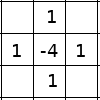
\includegraphics[scale = 0.8]{Images/Laplacian.png}
\end{center}

\subsubsection{Résolution de l'équation de Poisson} 
Soit $g(x,y) = S(x+1,y) + S(x-1,y)+ S(x,y+1) + S(x,y-1) - 			4\times S(x,y)$\\
Résoudre $\Delta I(x,y) = \Delta S(x,y)$ sur $\Omega$ est équivalent à résoudre :\\
\begin{center}
\begin{equation*}
    \left \{
    \begin{aligned}
    I(i+1,j) + I(i-1,j)+ I(i,j+1) + I(i, j-1) - 4\times 			I(i,j)= g(i,j)\\ pour (i,j)\in \Omega \\
    I(i,j) = T(i,j) \ pour \ (i,j) \in \partial \Omega
    \end{aligned}
    \right.
\end{equation*}
\end{center}
Nous devons donc résoudre un système à $M\times N $ inconnues.
\begin{equation}
\left\{
\begin{aligned}
I(1,1) = T(1,1)\\
I(3,2)+I(1,2)+ I(2,3)+I(2,1)-4I(2,2) =g(2,2) \\
I(3,3)+I(1,3)+ I(2,4)+I(2,2)-4I(2,3) =g(2,3)             \\
... \\
I(M,N-1)+I(M-2,N-1)+ I(M-1,N)+I(M-1,N-2)-4I(M-1,N-1) =g(M-1,N-1)\\
I(M, N) = T(M, N)
\end{aligned}
\right.
\end{equation}

Afin de résoudre ce système, il est plus facile de l'écrire sous forme matricielle. Nous devons donc résoudre un système de la forme AI = b et sa solution est ( en supposant que A est inversible ) :  $I = A^{-1}\times b$.
Avec : 
\begin{itemize}
\item A une matrice carrée de taille ($M\times N$, $M\times N$)
\item I un vecteur colonne de taille ($M\times N$,1)
\item b un vecteur colonne de taille ($M\times N$,1)
\end{itemize}
Voici donc à quoi ressemble le système que nous souhaitons résoudre :
\begin{center}

\begin{equation}
\left.
\begin{aligned}
\begin{pmatrix}
	-4 & 1 & 0 & ...& 0 & 1 & 0...&0& ... & 0\\
	1 & -4 & 1 & 0 & ... & 0 &1 &0&....&0\\
	0 & 1 & -4 & 1 & 0&... &0 &1 &0&...\\
	&...\\
	1 & 0 &... &1 &-4 &1 &0...& 0& 1 & 0\\
\end{pmatrix}
\begin{pmatrix}
I(1,1)\\
I(2,1)\\
...\\
I(1,2)\\
I(2,2)\\
....\\
I(M, N)
\end{pmatrix}
= 
\begin{pmatrix}
g(1,1)\\
g(2,1)\\
...\\
g(1,2)\\
g(2,2)\\
....\\
g(M, N)
\end{pmatrix}
\end{aligned}
\right.
\end{equation}
\end{center}

\subparagraph{Transformation de l'image}
Afin de pouvoir résoudre ce système, I doit être un vecteur colonne. Or dans notre cas, I est une matrice de taille (M,N). Le nouveau vecteur I, est la concaténation des colonnes de l'image I, comme ci dessous.

\subparagraph{Ecriture de la matrice du système}
La matrice A du système AI = b, est une matrice creuse, inversible. Nous verrons comment la remplir dans l'exemple ci-dessous.

\subparagraph{Ecriture de vecteur}
Après avoir calculé le Laplacien de l'image S, le vecteur b est obtenu en concaténant les colonnes de l'image $\Delta S$. 

\subsection{Exemple}
Considérons l'image S ci-contre que nous souhaitons coller. 
\begin{figure}[!h]
\centering

\includegraphics[scale=0.1]{Images/square.png}
\caption{Image à coller}
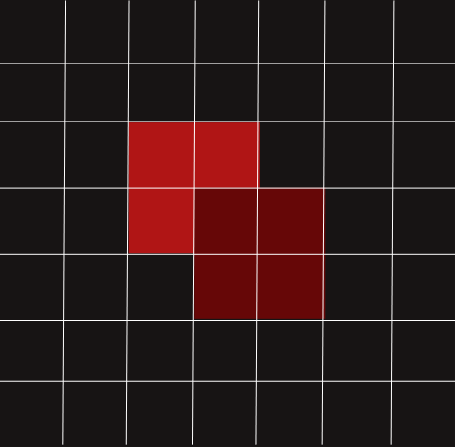
\includegraphics[scale=0.1]{Images/pix.png}
\caption{Vue grille pixel}
\end{figure}
Nous souhaitons ici coller les deux carrés rouge sur une image que nous nommerons T.   
\begin{figure}[!h]
\centering
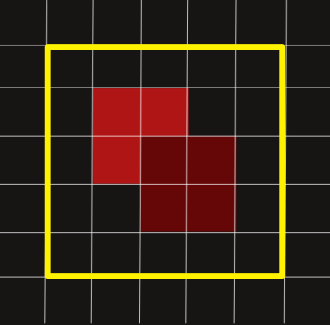
\includegraphics[scale=0.3]{Images/carre_selection.png}
\caption{Sélection à coller}
\end{figure}
Ici, notons $\Omega$, l'intérieur de la zone encadrée par la ligne verte, et des $\partial \Omega$, les pixels appartenant à $J /\ \Omega$

\begin{figure}[!h]
\centering
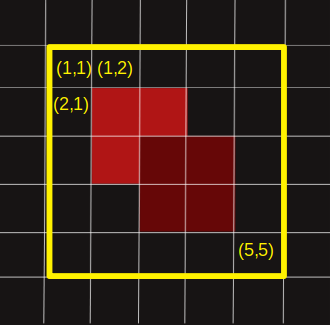
\includegraphics[scale=0.3]{Images/numerote.png}
\caption{Numérotation des pixels}
\end{figure}


\paragraph{Construction du système}
\begin{center}
\begin{equation}
\left\{
\begin{aligned}
I_{1,1} = T_{1,1}\\
...\\
I_{5,1} = T_{5,1}\\
I_{1,2} = T_{1,2}\\
\Delta I_{2,2} = \Delta S_{2,2}\\
\Delta I_{3,2} = \Delta S_{3,2}\\
\Delta I_{4,2} = \Delta S_{4,2}\\
...\\
\end{aligned}
\right.
\end{equation}
\end{center}
Avec $\Delta I(i,j) = U+D+L+R-4I(i,j)$.\\
En écrivant ce système sous forme matricielle la matrice A est la matrice $25\times 25$ ci-dessous :  

\begin{figure}[!h]
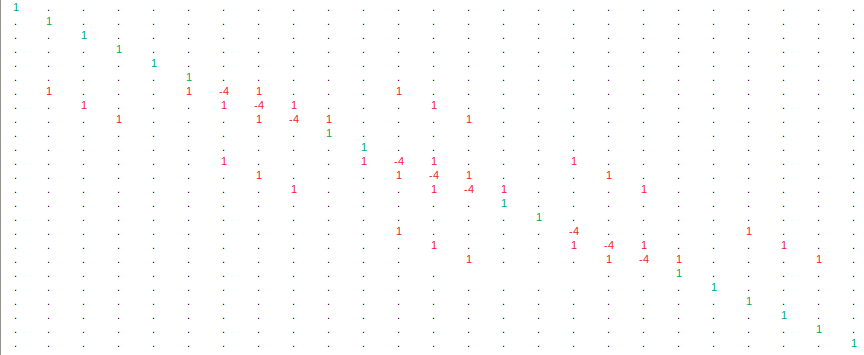
\includegraphics[scale=0.5]{Images/matrice.png}
\caption{Matrice du système}
\end{figure}

Le vecteur I est obtenu en concaténant les colonnes de la sélection, il est de taille($25\times 1$) : 
\begin{equation}
\begin{pmatrix}
I(1,1)\\
I(2,1)\\
...\\
I(5,1)\\
...\\
I(1,3)\\
...\\
I(5,3)\\
...\\
I(5,5)\\
\end{pmatrix}
\end{equation}
Enfin le vecteur b 

\begin{equation}
\begin{pmatrix}
T(1,1)\\
...\\
\Delta S(2,2)\\
...\\
T(5,2)\\
\Delta S(1,3)\\
...\\
T(5,3)\\
\Delta S(2,4)\\
...\\
\Delta S(4,4)\\
T(5,4)\\
...\\
T(5,5)\\
\end{pmatrix}
\end{equation}
La solution I, s'écrit sous la forme $I = A^{-1}b$.

